\section{Mathematical Model}
\subsection{Definitions}
A network-organized activator-inhibitor system can be defined in very close analogy to what one does for continuous media. 
In the network case, equations for the system are:
$$
\begin{cases}
\dot{u}_i(t) = f(u_i\, v_i) - \epsilon\,[L\,u(t)]_i \\
\dot{v}_i(t) = g(u_i\, v_i) - \epsilon\, \sigma [L\,v(t)]_i \\
\end{cases}
$$
Here, $\mathbf{u} = (u_1, \cdots u_N)$ and $\mathbf{v} = (v_1, \cdots v_N)$ are, respectively, the concentrations of the activator substance and the inhibitor substance on the $N$ nodes of the network. The reactions take place locally, on each node, and are encoded in the reaction terms $f(u_i\, v_i)$ and $f(u_i\, v_i)$. L is the laplacian matrix, defined as $L=D-A$. The diffusivity of the activator species is $\epsilon$, while that of the inhibitor is $\epsilon\,\sigma$, so that $\sigma$ is the ratio between them.

So far, the above are just the general equations of a reaction-diffusion system. In order to have a Turing mechanism, the reaction term need to satisfy the following basic requirements:
\begin{enumerate}
	\item Existence of a homogeneous equilibrium $(\overline{u},\, \overline{v})$ which is linearly stable in absence of diffusion (indeed, the key idea of the Turing model is that the instability is driven by diffusion, and appears only above a certain threshold function of the diffusion parameters) :
		$$
		\centering
		\begin{pmatrix}
			u_i(t) \\
			v_i(t)
		\end{pmatrix} \equiv  
		\begin{pmatrix}
			\overline{u} \\
			\overline{v}
		\end{pmatrix}
        \quad \forall i 
		\quad \text{where} \quad f(\overline{u}\,, \overline{v}) = g(\overline{u}\,, \overline{v})=0 \quad \text{and, given that}
		$$
		$$
		 \quad J(\overline{u}\,, \overline{v}) := 
		\begin{pmatrix}
 			f_u & f_v \\
 			g_u & g_v
 		\end{pmatrix}, \quad
 		\begin{cases}
 			\text{tr}(J)= f_u + g_v < 0\\
 			\text{det}(J) = f_u\cdot g_v f_v\cdot g_u>0
 		\end{cases}
		\text{(see \ref{app:bifurcation_diagram})}
		$$
	\item Correct qualitative behaviour of reactions in the neighborhood of the fixed point $(\overline{u},\, \overline{v})$: \newline
    the activator $u$ is supposed to enhance its own production and the production of the inhibitor $v$. Viceversa, the inhibitor $v$ is supposed to suppress the production of both the activator $u$ and itself. The functions $f,\, v$ need to reflect this behaviour, at least in a neighbourhood of the equilibrium $(\overline{u},\, \overline{v})$. Mathematically:
    \begin{center}
    \begin{minipage}{0.4\textwidth}
    \centering
    $$
           \begin{cases}
         f_u > 0,\quad f_v < 0 \\
         g_u >0,\quad  g_v <0 \\      
        \end{cases} 
    $$
    \end{minipage}
    \begin{minipage}{0.5 \textwidth}
    \centering
	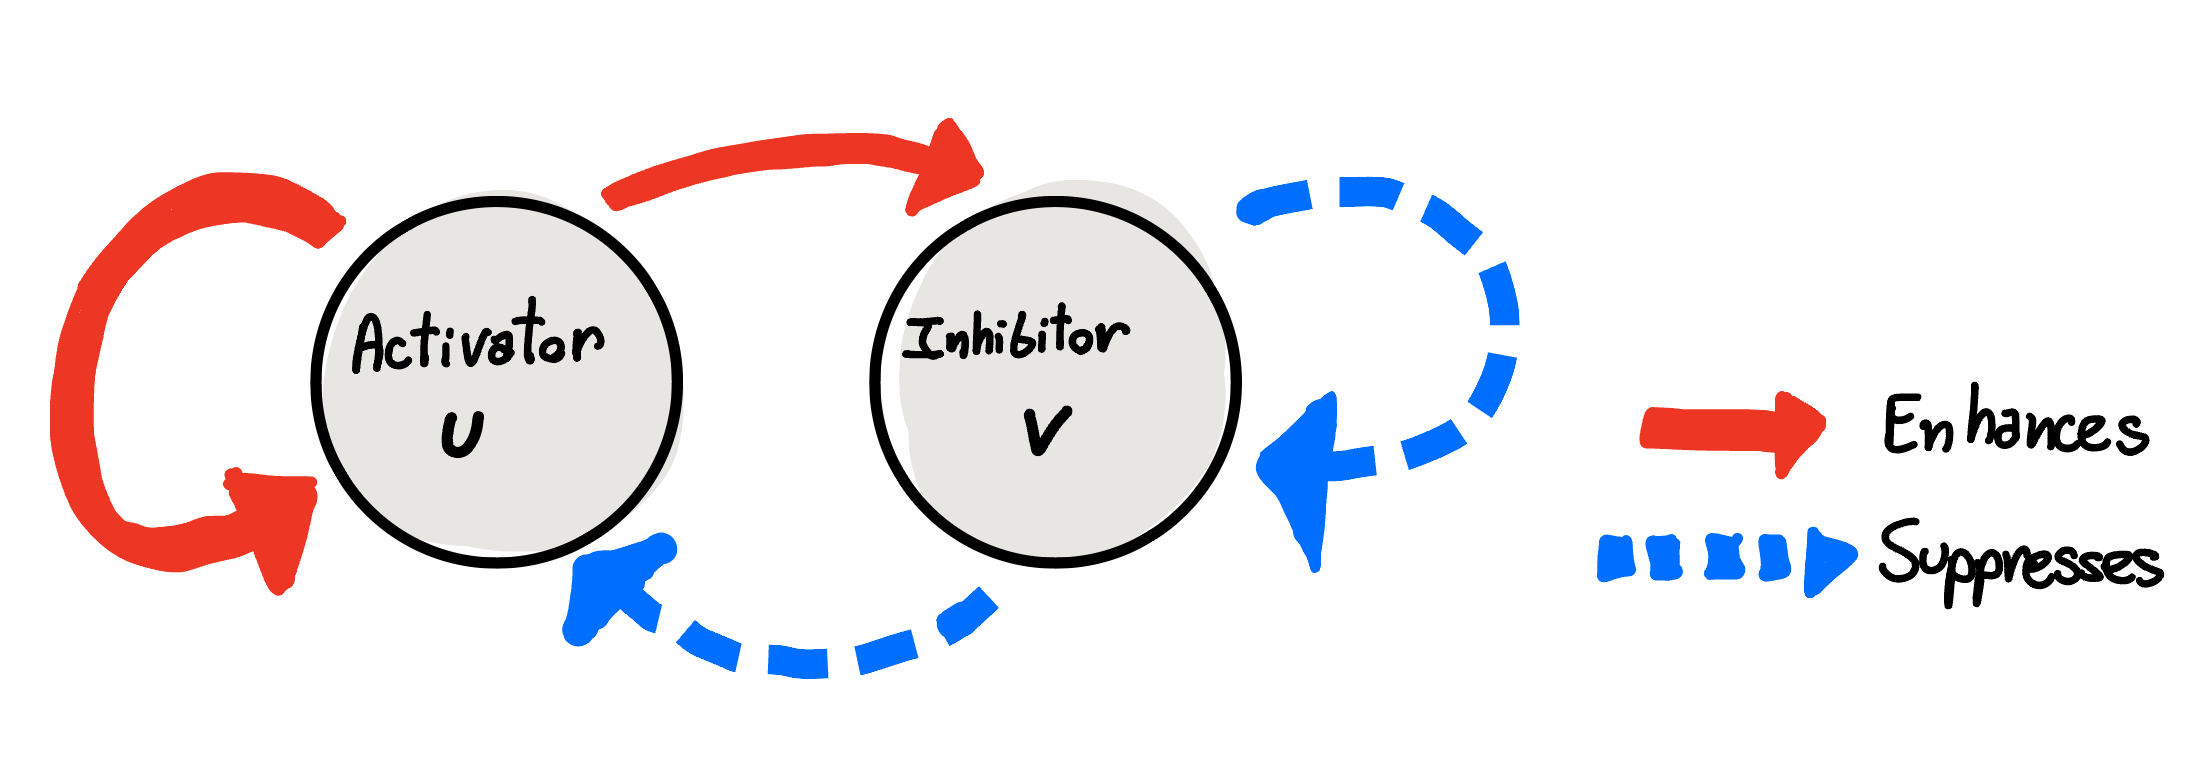
\includegraphics[width=0.9\textwidth]{images/diagram.jpeg}
 \label{fig:diagram}
    \end{minipage}
    \end{center}
\end{enumerate}
These requirements are just the same as in the case for the continuous medium. 
\subsection{Conditions for diffusion-driven instability}
Diffusion driven instability is investigated by means of linear stability analysis. A small random perturbation $\delta\,u_i,\, \delta\,v_i$ is added at each node, starting from the homogeneous equilibrium state. A linearized system of equations is obtained for the evolution of the perturbation:
\begin{equation}
    \begin{cases}
    u_i(t) = \overline{u} + \delta\, u_i(t)\\
    v_i(t) = \overline{v} + \delta\, v_i(t)
    \end{cases}
    \rightarrow 
    \begin{cases}
    \delta\, \dot{u}_i(t) \simeq \quad     f_u\, \delta u_i(t) +  f_v\, \delta v_i(t) - \epsilon\,[L\cdot (\overline{u}+ \delta u(t))]_i\\
    \delta\, \dot{v}_i(t) \simeq \quad 
    g_u \, \delta u_i(t) +  g_v \, \delta v_i(t) - \epsilon\,\sigma\,[L(\overline{v}+ \delta v(t))]_i
    \end{cases}
\end{equation}
But $L\,\overline{u} = L\,\overline{v} = 0$, since the constant vectors $u$ and $v$ are eigenvectors of the laplacian with eigenvalue zero.
In the case of a continuous medium, the perturbation is expanded as a Fourier series of plane waves. The rationale of this is that it makes the PDE turn into an eigenvalue problem.
In the network case, we instead write the perturbation as:
\begin{equation*}
    \begin{pmatrix}
    \delta u_i (t) \\
    \delta v_i (t) \\
    \end{pmatrix}
    =
    \begin{pmatrix}
        1 \\
        B_n \\
    \end{pmatrix}
    \cdot \sum_{n=1}^{N}\, c_n\,\Phi_i^{(n)}\, e^{\lambda_n\,t} \\
\end{equation*}
Where $\Phi^{(n)}$ is the $n-th$ eigenvector of the laplacian matrix $L$ and its corresponding eigenvalue is $\Lambda_n$ ($0=\Lambda_1 \leq \Lambda_2 \leq \cdots \Lambda_N$). The coefficients $\{c_n\}$ are determined by the initial conditions $(t=0)$. By doing this, the system of equations is turned into a $\Lambda -$dependent eigenvalue problem. In fact, if we plug the ansaltz 
\begin{equation*}
    \begin{pmatrix}
    \delta u_i (t) \\
    \delta v_i (t) \\
    \end{pmatrix}
    =
    \begin{pmatrix}
        1 \\
        B_n \\
    \end{pmatrix}
    \cdot  c_n\,\Phi_i^{(n)}\, e^{\lambda_n\,t} \\
\end{equation*}
into the linearized system of equations, we get:
\begin{equation*}
    \begin{pmatrix}
        \delta \dot{u}_i \\
        \delta \dot{v}_i \\
    \end{pmatrix}
    =
    \begin{pmatrix}
        f_u - \epsilon\,\Lambda_n & f_v \\
        g_u & g_v -\epsilon\,\sigma\,\Lambda_n \\
    \end{pmatrix}
    \cdot 
        \begin{pmatrix}
        \delta u_i \\
        \delta v_i \\
    \end{pmatrix}
\end{equation*}
\begin{equation*}
    \rightarrow
        \lambda_n \cdot
        \begin{pmatrix}
        1 \\
        B_n\\
    \end{pmatrix}
    =
    \begin{pmatrix}
        f_u - \epsilon\,\Lambda_n & f_v \\
        g_u & g_v -\epsilon\,\sigma\,\Lambda_n \\
    \end{pmatrix}
    \cdot 
        \begin{pmatrix}
        1 \\
        B_n\\
    \end{pmatrix}
\end{equation*}
Or, in compact form:
\begin{equation*}
    \lambda_n\, \mathbf{v}_n = M(\Lambda_n,\,\sigma,\,\epsilon)\, \mathbf{v}_n
\end{equation*}
The differences between the network case and the continuous medium case end here. From now on, the steps are exactly the same. We are looking for instability, thus we want to find the range of parameters $(\sigma,\, \epsilon)$ that produce $\mathcal{R}e\{\lambda_{\pm}(\Lambda)\}>0$ for a positive range of $\Lambda$'s. \\
First, we must have that at least one of the following holds
\begin{equation*}
    \begin{cases}
        \text{det}[M(\Lambda,\,\sigma,\,\epsilon)]<0 \\
        \text{tr}[M(\Lambda,\,\sigma,\,\epsilon)]> 0 \\
    \end{cases}
\end{equation*}
But $\text{tr}[M(\Lambda,\,\sigma,\,\epsilon)] = \text{tr}[J] - \epsilon\, \Lambda\, (1+\sigma)<0$ because the homogeneous state is a stable equilibrium, then the only possibility is that $\text{det}[M(\Lambda,\,\sigma,\,\epsilon)]< 0$. \\
Some quick boring algebra now:
\begin{equation*}
    \text{det}[M(\Lambda,\,\sigma,\,\epsilon)] = \epsilon^2\,\sigma\,\Lambda^4 - \epsilon\,(g_v +\sigma\,f_u) \Lambda + \text{det}[J] \overset{!}{\leq} 0 \quad \text{for some}\, \Lambda >0
\end{equation*}
\begin{minipage}{0.6\textwidth}
This is a parable of kind $y = a\,x^2 - b\,x + c$ with  $(a,\,b,\,c>0)$, so the minimum is reached at coordinates $(x_{min},\,y_{min}) = (\frac{b}{2\,a}\,, c-\frac{b^2}{4\,a})$. The parable touches the $x$ axis ($y_{min}\leq 0$) $\iff$ $\Delta^2 = b^2-4\,a\,c \geq 0$.
\end{minipage}
\hfill
\begin{minipage}{0.38\textwidth}
    \centering
    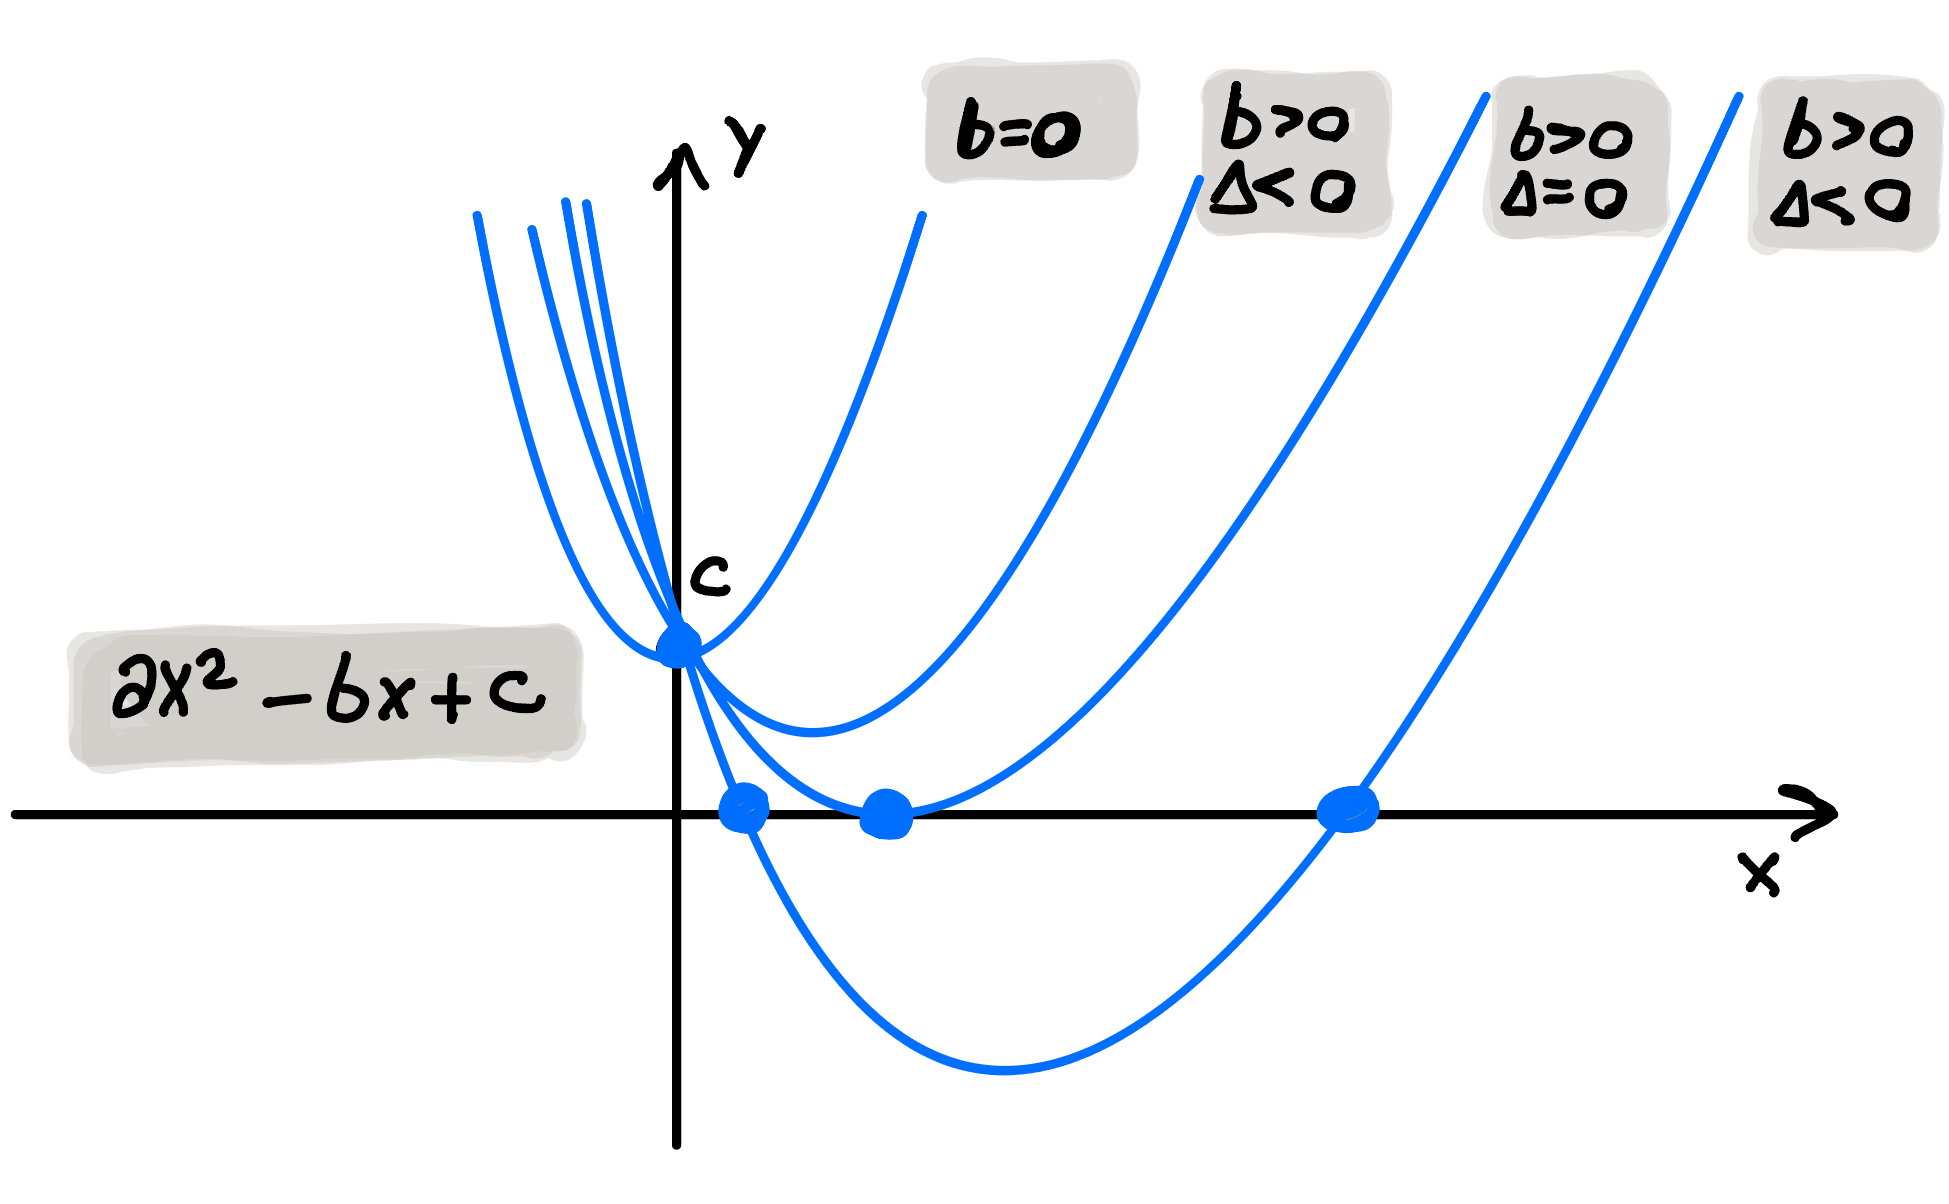
\includegraphics[width=\textwidth]{latex_source/images/parable.jpeg}
\end{minipage}
\newline
We require:
\begin{equation*}
    \begin{cases}
        x_{min}(\epsilon,\,\sigma)>0 \\
        y_{min}(\epsilon,\,\sigma)\leq 0 \\
    \end{cases}
    \quad
        \begin{cases}
        \epsilon\,(g_v +\sigma\,f_u) > 0 \\
        [\epsilon\,(g_v +\sigma\,f_u)]^2 \geq 4\,\epsilon^2\,\sigma\,\text{det}[J] \\
    \end{cases}
\end{equation*} 
From the first one, we notice that there exists a minimum value threshold for $\sigma > \sigma_{min}= \frac{|g_v|}{f_u}$. Also, since $\text{tr}\,[J]=(-|g_v| +f_u)<0$, then $\sigma_{min}> 1$: a necessary (but still not sufficient) condition for pattern initiation is that the inhibitor diffuses faster than the activator.
\begin{equation*}
    \begin{cases}
        \sigma > \sigma_{min} >1  \\
        f_u^2\,\sigma^2 + 2\,(f_u\,g_v-2\,\text{det}[J])\,\sigma + g_v^2 \geq 0 
    \end{cases}
    \quad 
    \begin{cases}
    \sigma > \sigma_{min} >1  \\
    \sigma < \sigma_{-}(<\sigma_{min}) \quad \text{or} \quad  \sigma > \sigma_{+}\\
    \end{cases}
\end{equation*} 
Where $\sigma_{\pm}$ are the roots of the quadratic equation:
\begin{equation*}
    \sigma_{\pm} = \frac{(f_u\,g_v - 2\,f_v\,g_u)\,\pm 2\,\sqrt{f_v\,g_u\,(f_v\,g_u-f_u\,g_v))}}{f_u^2}
\end{equation*}
The function $y_{min}(\sigma)$ reaches its maximum for $\sigma=\sigma_{min}$ and goes to $-\infty$ for both $\sigma\rightarrow0^{+}$ and $\sigma\rightarrow +\infty$. Also, the lower-branch root $\sigma_{-}$ is below the threshold value $\sigma_{min}$. Then, both our requirements are satisfied if and only if $\sigma>\sigma_{+}$. In summary, the necessary and sufficient condition for instability is
\begin{equation*}
 \sigma > \sigma_c :=  \frac{(f_u\,g_v - 2\,f_v\,g_u)\, + 2\,\sqrt{f_v\,g_u\,(f_v\,g_u-f_u\,g_v))}}{f_u^2}
\end{equation*}
\textbf{Critical eigenvalue and graph finite size effect} \newline
The critical eigenvalue $\Lambda$ is determined for give $\epsilon$:
\begin{equation}
\label{eq:critical_eigenvalue}
    \Lambda_c(\epsilon) := \Lambda(\sigma=\sigma_c,\,\epsilon) = \frac{g_v + \sigma_c\,f_u}{2\,\epsilon \,\sigma_c} = (\cdots) = \frac{1}{\epsilon}\,\sqrt{\frac{\text{det}[J]}{\sigma_c}}
\end{equation}
For $\sigma$ above the critical threshold, a finite range [$\Lambda_1\,\Lambda_2$] centered around $\Lambda_c$ appears where the corresponding mode is unstable. However, the eigenvalue spectrum of the laplacian matrix is not continuous. Instability will appear if there are allowed modes that fall inside this range.
In particular, the eigenvalue spectrum of the laplacian is bounded above for a graph of finite size. If the mobility $\epsilon$ is small enough, the critical eigenvalue could lay beyond the largest eigenvalue of the graph, and instability would not occur.
This finite-size effect appears also in the case of a continuous medium. There, instability cannot occur when the spatial domain is too small and the largest allowed wavelength is less than the critical wavelength.
\medskip \newline
\textbf{Dispersion relation $\lambda(\Lambda;\, \sigma,\,\epsilon)$} \newline
Finally, the growing rate of the unstable mode, $\lambda_n = \lambda(\Lambda_n)$ is calculated from the caractheristic polynomial of $M(\Lambda_n, \sigma,\,\epsilon)$:
\begin{equation*}
    p(\lambda) = (\lambda-\lambda_1)\cdot(\lambda-\lambda_2) = \lambda^2 - \text{tr}[M(\Lambda,\,\sigma,\,\epsilon)]\cdot \lambda + \text{det}[M(\Lambda,\,\sigma,\,\epsilon)]
\end{equation*}
\begin{align*}
    \lambda_{\pm} &=\frac{1}{2}\,\left[\text{tr}[M]\pm \sqrt{\text{tr}[M]^2-4\,\text{det}[M]}\right] = \frac{1}{2}\,\left[-|\text{tr}[M]|\pm \sqrt{\text{tr}[M]^2-4\,\text{det}[M]}\right] \\
    &= \frac{1}{2}\, \left[\left[f_u + g_v - (1+\sigma)\,\epsilon\,\Lambda\right] + \sqrt{4\,f_v\,g_u + \left[f_u - g_v -(1-\sigma)\,\epsilon\,\Lambda\right]^2}\right]
\end{align*}
In the instability region, $\text{tr}[M] <0$ and $\text{det}[M]<0$, then eigenvalues are real and distinct. Also, the lower branch is always negative so we are not interested in it. By comparison with the graph of $\text{det}[M(\Lambda,\,;\epsilon,\,\sigma]$, we get the qualitative dependence of $\lambda$ from $\Lambda$, commonly called "dispersion relation".
\newpage

